\chapter{RoboCup2D}
    % ``Was ist RoboCup'' \\
    % ``Was für Ligen gibt es'' \\
    % ``Was für eine Domäne ist es im Vergleich zu anderen'' \\
    % \\
    RoboCup ist ein Fußball Simulator, der seine Anfänge in 1993 in Japan, Tokyo gefunden hat. Eine Gruppe von Forschern, inklusive Minoru Asada, Yasuo Kuniyoshi und Hiroaki Kitano, haben als einen Wettbewerb unter dem Namen \textbf{Robot J-League} gestartet. Der Name stammt von einer professionellen japanischen Fußball Liga \cite{hfo-history}.\\
    \\
    Nach einem Monat haben sie jedoch weltweit überwältigendes Feedback bekommen und haben die Initiative als internationales Projekt weitergeführt, daher kam die Umbenennung zur \textbf{Robot World Cup Initiative}, kurz RoboCup. \\
    % \textit {(source: http://www.robocup.org/about-robocup/a-brief-history-of-robocup/)} \\
    \\
    Die RoboCup Initiative betreibt derzeit sechs große Wettbewerbe, die sich jeweils wieder in Ligen und Subligen aufteilen lassen. Darunter fällt \textbf{RoboCup Soccer}, \textbf{RoboCup Rescue Rescue}, \textbf{RoboCup Junior}, \textbf{RoboCup Logistics}, \textbf{RoboCup @ Work} und \textbf{RoboCup @ Home}. Unsere Implementierung fällt in die Subliga \textbf{2D Soccer Simulation}, in der es darum geht in einer zweidimensionalen Welt zwei Fußballmannschaften gegeneinander antreten zu lassen.\\
    \\
    Die Aufgabe, die wir angehen, gehört zu einem Fragement von RoboCup2D, genannt \textbf{Half Field Offense}.\\
    \begin{figure}[htbp]
        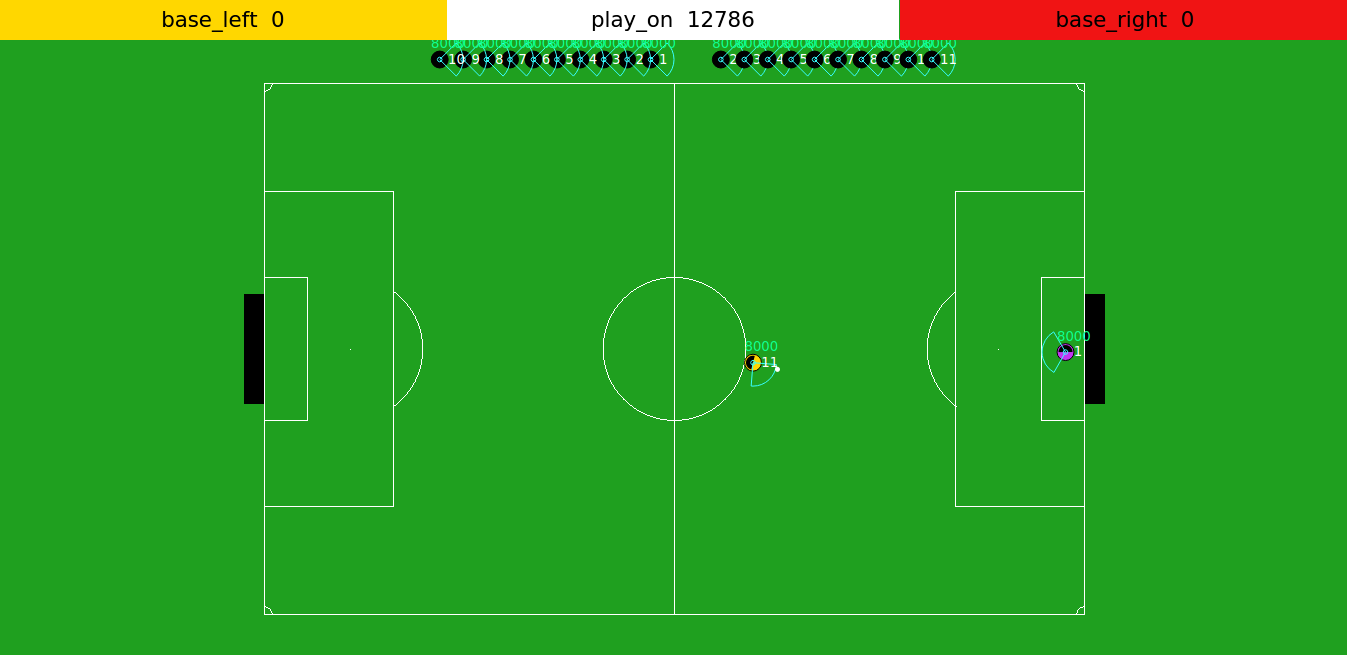
\includegraphics[width = 1.0\textwidth, center]{../pictures/full-field.png}
        \caption{Screenshot von dem gesamten Spielfeld von RoboCup2D \label{fig:somelabel}}
    \end{figure}

    \section{Half Field Offense}

        Die Domäne Half Field Offense grenzt das Spielfeld auf eine Hälfte ein, sodass wir 4 Angreifer und 3 Verteidiger + Torwart haben. Diese Einschränkung vereinfacht den Such- und Zustandsraum immens und erlaubt trotzdem noch eine Wiederverwendbarkeit der Agenten, wenn eine vollständige Mannschaft aufgebaut wird.\\
        \\
        In unserer Implementierung haben wir lediglich ein 1vs1 Szenario, also ein Angreifer gegen ein Torwart. Die Modellierung erlaubt dennoch ein nahtlosen Skalierung auf ein 4vs4 Szenario, sodass weitere Parametrisierung ohne viel Aufwand ausprobiert werden können.\\

        \begin{figure}[htbp]
            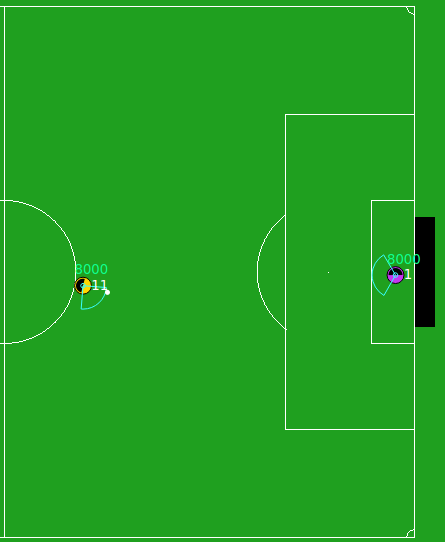
\includegraphics[width = 0.7\textwidth,height = 0.6\textheight, center]{../pictures/half-field.png}
            \caption{Screenshot von dem Spielfeld für den Subtask HFO \label{fig:somelabel}}
        \end{figure}
        \noindent
        Im Folgenden wird die Domäne samt Zustandsraum und Aktionen erklärt, sowie ihren Einschränkungen für die Anwendung von Machine Learning Algorithmen.\\
        % \cite{ http://www.cs.utexas.edu/users/ai-lab/?hausknecht:aamasws16 }
\newpage
        \subsection{Zustandsraum} \label{statespace-definition}
            % ``Unterschiedliche Zustandsräume, kommt drauf an wie viele Spieler aufm Feld sind (zitat vom HFO Paper)''\\
            % ``Angepasst für Maschinen (zitat HFO)'' \\
            % ``Umrechnung für Menschen'' \\
            % ``Fullstate flag''
            Der Zustandsraum der HFO Domäne kann in den \textbf{High Level State} und den \textbf{Low Level State} aufgeteilt werden. Der Unterschied liegt in der Dimensionalität, da man aus dem Low Level State den High Level State ableiten kann. Die Zustandsräume werden durch folgende Formeln definiert:\\
            
            \begin{mdframed}
            \textit{Sei T die Anzahl der Teammitglieder, O die Anzahl der Gegner:}
            \begin{center}
                $dim($\textit{High Level State}$)$ $ := 10 + 6T + 3O \hspace{10mm} $ \\
                $dim($\textit{Low Level State}$)$  $ := 58 + 8T + 8O \hspace{9mm} $ \\
            \end{center}
            \end{mdframed}
%            \textit{(Frage: Alles vom Paper abschreiben oder referenzieren?)} \\
            \hfill  \\
            In unserem 1vs1 High Level Setting haben wir damit 13 Zustandsparameter. Vier von diesen Parametern gehören zu dem Torwart, aber da seine Position implizit durch andere Eigenschaftn gegeben ist, beachten wir sie nicht. Redundante Information würde den Suchraum unnötig aufblähen und die Suche verlängern. Deshalb wurden nur die folgenden 9 Zustände bereitgestellt:

            \begin{table}[H]
                \begin{center}
                \hspace*{-0.75cm}
                \begin{tabular}{ |l|c|c|c|c| } 
                    \hline
                    \hfill Zustandsbeschreibung                          & Winkel & Boole'sch & Lage & Anderes \\ \hline
                    x-Koordinaten                                        & \hfill & \hfill    &      & X       \\ \hline
                    y-Koordinaten                                        & \hfill & \hfill    &      & X       \\ \hline
                    Sichtrichtung                                        & X      & \hfill    &      & \hfill  \\ \hline
                    Nähe zum Ball                                        & \hfill & \hfill    & X    & \hfill  \\ \hline
                    Winkel zum Ball                                      & X      & \hfill    &      & \hfill  \\ \hline
                    Kann eine Ballaktion ausgeführt werden               & \hfill & X         &      & \hfill  \\ \hline
                    Winkel zum Mittelpunkt des Tors                      & X      & \hfill    &      & \hfill  \\ \hline
                    Größte offene Winkel zwischen Torwart und Torpfosten & X      & \hfill    &      & \hfill  \\ \hline
                \end{tabular}
                \end{center}
%                \caption{Zustandsraum von HFO 1vs1 \label{fig:somelabel}}
            \end{table}

            % \hspace*{-1.5cm}
            % \textit{(Muss hier eine Erklärung wie der Zustand kodiert war hin, also Normalisierung der Winkel?\\
            % \hspace*{-1.5cm} Wäre dann eigentlich abschreiben ab 15.1.1 von https://github.com/LARG/HFO/blob/master/doc/manual.pdf)}
            % (src: https://github.com/LARG/HFO/blob/master/doc/manual.pdf ab 15.1.1)
            \noindent
            Der Zustand kann in 4 Kategorieren unterteilt werden, die alle auf den Wertebereich von $[ -1, +1 ]$ reduziert wurden.

            \subsubsection*{Winkelkodierung}
                Die Winkel sind im Bereich von $[0, \pi]$ und durch folgende Formel auf den Bereich $[-1, +1]$ transformiert \footnote[1]{Formel sind aus dem E-Mail Verkehr mit dem Entwickler entstanden}:

                \begin{mdframed}
                    Sei $f : [0,\pi] \rightarrow [-1, +1]$ die Kodierungsfunktion \\
                    \hspace*{5mm} $g : [-1, +1] \rightarrow [0, \pi]$, die Inverse: \\[4mm]
                    \hspace*{10mm} \Resize{4.5cm}{$f(x) = (\frac{x}{\pi} - 1) \cdot 2$}
                    \hspace*{20mm} \Resize{4.5cm}{$g(x) = (\frac{x}{2} + 1) \cdot \pi$}
                \end{mdframed}
                

            \subsubsection*{Boole'sche Kodierung}
                Die boole'schen Werte sind binär und $-1$ entspricht $false$ und $1$ entsprechend $true$.

            \subsubsection*{Lagekodierung}
                Die Lagekodierung ist normalisiert auf der maximale diagonale Länge des Spielfelds die durch $max_{l} = \sqrt{l^2 + w^2}$ gegeben ist, wobei $l$ die Länge und $w$ die Breite ist. In dem Fall für HFO, entspricht sie $sqrt(2^2 + 2^2) ~= 2.82$. Die dafür Formeln sind: \\

                \begin{mdframed}
                Sei $f : [-max_{l}, max_{l}] \rightarrow [-1, +1]$ die Kodierungsfunktion \\
                    \hspace*{5mm} $g : [-1, +1] \rightarrow [-max_{l}, max_{l}]$, die Inverse: \\[4mm]
                    \hspace*{25mm} \Resize{3.5cm}{$f(x) = \frac{x}{max_{l}}$}
                    \hspace*{20mm} \Resize{3.5cm}{$g(x) = x \cdot max_{l}$}
                \end{mdframed}

            \subsubsection*{Anderes}
                Unter diese Kategorie fallen nur die x- und y-Koordinaten und sind trivialerweise im Bereich von $[-1, +1]$, weil das die Grenzen des Spielfelds sind.

\newpage
        \subsection{Aktionsraum} \label{actionspace-definition}
            % ``Gibt 6 nicht parametrisierte Aktionen, die wir benutzt haben''\\
            % ``Gibt noch andere parametrisierte''
            Es gibt 8 parametrisierte und 6 nicht parametrisierte Aktionen. Wir haben die Algorithmen auf 5 der Aktionen trainiert die nicht parametrisiert sind. Die Aktion \textit{CATCH} ist für Angreifer illegal und wurde deshalb weggelassen. Die folgende Aufzählung beschreibt alle Aktionen \cite{hfo}:

            \begin{multicols}{2}
                \textbf{Parametrisierte}
                \begin{itemize}
                    \item Dash(power, degrees)
                    \item Turn(degrees)
                    \item Tackle(degrees)
                    \item Kick(power, degrees)
                    \item Kick\_To(x-coords, y-coords, speed)
                    \item Move\_To(x-coords, y-coords)
                    \item Dribble\_To(x-coords, y-coords)
                    \item Pass(playernumber)
                \end{itemize} \par
                \textbf{Nicht parametrisierte}
                \begin{itemize}
                    \item Move
                    \item Shoot
                    \item Dribble
                    \item Intercept
                    \item Catch
                    \item No-Op
                \end{itemize}
            \end{multicols}

            \subsubsection*{Aktion: Move}
            \textit{Move} repositioniert den Agenten nach der vorprogrammierten Strategie von \textit{Agent2D} und funktioniert nur dann, wenn der Spieler den Ball nicht hat.

            \subsubsection*{Aktion: Shoot}
            Diese Aktion versucht den Ball mit der besten Parametern für die Aktion \textit{Kick\_To} aufzurufen, sodass ein Tor geschossen wird. 

            \subsubsection*{Aktion: Dribble}
            Der Agent benutzt kurze \textit{Kick\_To} und \textit{Move} Sequenzen um in die Nähe des Tores zu laufen.

            \subsubsection*{Aktion: Intercept}
            Der Agent versucht in die Nähe des Balls zu laufen indem er die Geschwindigkeit vom Ball in Betracht zieht. Diese Aktion ist effektiver als \textit{Move}.

            \subsubsection*{Aktion: No-Op}
            Wenn diese Aktion gewählt wird, macht der Agent nichts.

            \subsubsection*{Abfrage der Aktionen}
            Jedes Spiel hatte eine maximale Laufzeit die in Frames aufgeteilt wird und jeder Agent pro Frame gefragt, welche Aktion er ausführen will. Wenn über längere Zeit keine Antwort von dem Agenten kommt, wird automatisch die No-Op Aktion ausgeführt.


        \subsection{Einschränkungen}
            % ``Sparse Fitness''                 \\
            % ``Simulation Learning''            \\
            % ``Hochdimensional Kontinuierlich'' \\
            % ``Auch genannt Black Box RL''
            Diese Domäne hat besondere Einschränkungen, die es zu einem schwierigen Problem machen. Zum einen haben wir keine Möglichkeit in die Zukunft zu schauen um herauszufinden wie gut eine Aktion für einen bestimmten Zustand war. Stattdessen müssen wir uns auf das Resultat der Simulation verlassen, dass uns lediglich am Ende sagt ob ein Tor geschossen wurde. \\[2mm]
            \noindent
            Zum anderen ist ein Spiel eine Abfolge von mehreren hundert Aktionen die alle gemeinsam bewertet werden und deshalb ist es unmöglich eine Fragmentierung in Teilziele zu schaffen. \\[2mm]
            \noindent
            Zusätzlich zum spärlichen Signal ob wir ein Tor geschossen haben, kommt der kontinuierliche 9-dimensionale Zustandsraum den wir mit normalverteiltem Rauschen empfangen haben.

%             enn man sie mit herkömmlichen Machine Learning Tasks vergleicht \textit{(Vergleich Moonrover, Roboterarm etc.)}. Zum einen erlaubt sie uns wegen der Implementierung nicht in die Zukunft zu propagieren und zu schauen wie gut eine Entscheidung ist. Wir haben eine Simulation die erst nachdem ein Spiel fertig ist ein Fitnesssignal sendet und wir daraufhin abzuleiten müssen ob die lange Aktionsketten die wir ausgeführt haben uns zum Erfolg führten. Diese Eigenschaft nennt sich \textbf{sparse Fitness} und findet sich in Beispielen wie \textit{(Zitat)}

%            \begin{center} \textit{(Simulation based learning)} \end{center}
%            \begin{center} \textit{(Kontinuierlicher Zustandsraum, hohe Abstraktion)} \end{center}
            % (cite https://gym.openai.com/docs/rl#black-box-optimization-and-the-cross-entropy-method)
\newpage

    \section{Implementierung der Algorithmen}
        In diesem Abschnitt schauen wir uns die Parametrisierung der Algorithmen und den Aufbau der Simulation genauer an. Dafür waren die folgenden drei Programme zuständig:

        \subsubsection*{Simulationsserver}
        Der Simulationsserver ist in C++ geschrieben und wurde aus \cite{hfo} übernommen. Er wird durch Flags beim Starten parametrisiert. 

        \subsubsection*{Agenten}
        Die Agenten sind in Python geschrieben und stellen eine Erweiterung von einem der Beispielskripte dar \cite{hfo}. Diese Prozesse werden mit eigenen Kommandozeilenparametern, die ihnen sagen welcher Spieler sie sind, wie sie die Kodierung des KNNs benutzen, um damit das Netz zu befüllen.

        \subsubsection*{Koordinator}
        Der Koordinator ist für die Umsetzung des GAs und den jeweiligen Kodierungen zuständig, startet den Server, die Agenten Skripte und überwacht die Simulation. Er ist, wie alle folgenden Codebeispiele, in Haskell geschrieben.


        \subsubsection*{Rahmenbedingungen für die Simulation}
        Jede Simulation bestand aus 300 Generationen und jedes Team hat pro Generation 25 Spiele gespielt. Ein Spiel (Episode) war maximal 500 Sekunden lang und wenn der Ball 50 Sekunden lang nicht berührt wurde, zählt das Spiel als verloren. Die Algorithmen die Selektion und Mutation unterstützen, wurden mit folgenden Parametern gestartet:
        \hfill \\
        \begin{center}
            \begin{tabular}{ |c|c| } 
                \hline
                Generationen       & $300$  \\ \hline
                Populationsgröße   & $50$   \\ \hline
                Teamepisoden       & $25$   \\ \hline
                Episodenzeit       & $500s$ \\ \hline
                Ball nicht berührt & $50s$  \\ \hline
                Selektion $\alpha$ & $25\%$ \\ \hline
                Mutation $\beta$   & $10\%$ \\ \hline
            \end{tabular}
        \end{center}

\newpage

        \subsection{Wahrscheinlichkeitsverteilung von Aktionen}

            Der erste Algorithmus hat als Kodierung der Individuen eine diskrete Wahrscheinlichkeitsverteilung über 5 Aktionen benutzt. Wenn der Agent gestartet wurde samplet er jeden Zeitschritt ohne Wissen über jeglichen Zustand aus dieser Verteilung raus. 

            \subsubsection*{Kodierung}

            \begin{figure}[H]
                \begin{mdframed}
                    Sei das Set von allen Aktionen $ X := $ \{Move, Shoot, Dribble, Intercept, No-Op\}, \\
                    $P(x)$ die Wahrscheinlichkeit dass $x$ eintrifft, dann gilt: \\[2mm]
                    \hspace*{25mm} \Resize{8cm}{$\forall x \in X: P(x) \geq 0 \;\;\land\;\; \sum_{x \in X}^{} P(x) = 1$}
                \end{mdframed}
                \renewcommand{\figurename}{Lemma}
                \caption{\label{kodierung} Regeln für die Wahrscheinlichkeitsverteilung der Aktionen}
            \end{figure}

%            \subsubsection*{Kreuzung}
%            Die Kreuzung wurde auf zwei verschieden Arten umgesetzt, wobei sie im Vergleich an der vollständigen Simulation gleich gut abgeschnitten haben.

            \subsubsection*{Generierung der Individuen}
            Für die Generierung von einer Wahrscheinlichkeitsverteilung über $n$ Aktionen werden $n-1$ zufällige Zahlen erstellt, sortiert und es wird jeweils eine $0$ von vorne und eine $100$ am Ende angehängt.

            \begin{mdframed}
            \begin{minted}[escapeinside=||, linenos]{haskell}
> let n = 5
> take (n-1) <\$> getRandomRs (0,100)
[87, 15, 55, 38]
> sort it
[15, 38, 55, 87]
> 0 : it ++ [100]
[0, 15, 38, 55, 87, 100]
            \end{minted}
            \end{mdframed}
            \noindent
            Um die Verteilung zu erstellen werden die Zahlen dupliziert, um ein Element nach rechts verschoben und nach dem Index voneinander abgezogen.
            \begin{mdframed}
            \begin{minted}[escapeinside=||, linenos]{haskell}
> let l1 = [0, 15, 38, 55, 87, 100]
> drop 1 l1
[15,38,55,87,100]
> let l2 = it
> {-
  [15, 38, 55, 87, 100]
- [ 0, 15, 38, 55,  87, 100]
= [15, 23, 17, 32,  13]
-}
> zipWith (-) l2 l1
[15, 23, 17, 32, 13]
> sum it
100
            \end{minted}
            \end{mdframed}
            \noindent
            Damit haben wir eine Wahrscheinlichkeitsverteilung über 5 Aktionen und können uns sicher sein dass sie aufsummiert immer $100$ ergibt.

            \subsubsection*{Kreuzung Version 1}
            Wir haben zwei verschiedene Kreuzungsmethoden ausprobiert die sich in unserer Simulation als gleichwertig herausgestellt haben.
            Die erste Methode wurde mit den Listen umgesetzt, aus denen sie generiert wurden (die jeweils die 0 und 100 angehängt bekommen haben). Dafür wurde elementweise der Durchschnitt berechnet und daraus entsteht dann eine neue Generatorliste aus der sich die Verteilung berechnen lässt.
            \begin{mdframed}
            \begin{minted}[escapeinside=||, linenos]{haskell}
> let individualA = [0, 15, 38, 55, 87, 100]
> let individualB = [0, 7, 22, 35, 51, 100]
> zipWith (\x y -> (x + y) `div` 2) individualA individualB
[0, 11, 30, 45, 69, 100]
            \end{minted}
            \end{mdframed}
            \subsubsection*{Kreuzung Version 2}
            Die zweite Methode hat beide Verteilungen genommen, die Wahrscheinlichkeiten für jeweiligen Aktionen addiert und folgendermaßen normalisiert:\\
            \noindent
            \begin{figure}[H]
                \begin{mdframed}
                    Seien $\mathcal{A, B}$ diskrete Wahrscheinlichkeitsverteilungen, $l = |\mathcal{A}|$, $i \in \{1 ... l\}$:\\[4mm]
                    \hspace*{40mm}\Resize{6.5cm}{$\mathcal{C} := \{ \frac{(a_i + b_i)}{l} \; | \; a_i \in \mathcal{A}, b_i \in \mathcal{B}\}$} \\[4mm]
                    dann ist $\mathcal{C}$ ist ihre Verknüpfung.
                \end{mdframed}
                \renewcommand{\figurename}{Definition}
                \caption{\label{norm-prop} Kreuzungsmethode 2 für Wahrscheinlichkeitsverteilungen}
            \end{figure}

            \subsubsection*{Mutation}
            Die Mutation wurde auch auf zwei verschiedene Weisen umgesetzt. Im Kern ist jedoch die Funktion die das $\delta$ benutzt und es mit zufälligen Vorzeichen in die Anzahl der Aktionen $n$ aufgeteilt. Man kann sich das $\delta$ als Veränderungsfaktor vorstellen, je höher er ist, umso unterschiedlicher wird die Wahrscheinlichkeitsverteilung.
            \begin{mdframed}
                \begin{minted}[escapeinside=||, linenos]{haskell}
> let delta = 20                            > let delta = 100
> splitDelta delta 5                        > splitDelta delta 4
[-4, +4, +4, -4, -4]                        [-25, +25, +25, -25]
                \end{minted}
            \end{mdframed}

            \subsubsection*{Mutation Version 1}
            Wir teilen das $\delta$ in $n-1$ Teile auf, fügen eine $0$ von vorne und $100$ von hinten hinzu und addieren sie zu der Generatorliste der Verteilung. Diesmal müssen wir jedoch die Zahlen per Hand auf den Bereich von $0 - 100$ begrenzen.
            \begin{mdframed}
            \begin{minted}[escapeinside=||, linenos]{haskell}
> let delta = 100
> splitDelta delta 4
[-25, +25, +25, -25]
> let mutGen = 0 : it ++ [100]
> let child = [0, 14, 31, 49, 75, 100]
> {-
  [0, -25, +25, +25, -25, 100]
+ [0,  14,  31,  49,  75, 100]
= [0, -11,  56,  74,  50, 200]
min 0
  [0,   0,  56,  74,  50, 200]
max 100
  [0,   0,  56,  74,  50, 100]
sort
  [0,   0,  50,  56,  74, 100]
-}
> sort $ zipWith (((max 0 . min 100) .) . (+)) child mutGen
[0,0,50,56,74,100]
            \end{minted}
            \end{mdframed}
            Aus diesem Generator kann wieder eine Wahrscheinlichkeitsverteilung erstellt werden.

            \subsubsection*{Mutation Version 2}
            Für die zweite Variante der Mutation spalten wir das $\delta$ in $n$ Teile, summieren sie elementweise mit der Verteilung, überprüfen auf die Grenzen von [$0,100$] und normalisieren sie wie in Kreuzung Version 2.
            \begin{mdframed}
            \begin{minted}[escapeinside=||, linenos]{haskell}
> let delta = 50
> splitDelta delta 5
[-10, +10, +10, -10, -10]
> let mutGen = it
> let child = [15, 8, 34, 21, 22]
> zipWith (((max 0 . min 100) .) . (+)) child mutGen
[5,18,44,11,12]
> normalizeDist it
[5,20,48,12,15]
            \end{minted}
            \end{mdframed}
            Damit bekommen wir die mutierte Wahrscheinlichkeitsverteilung zurück.

\newpage

        \subsection{Agentenstrategien als KNN mit DCT} \label{knn-dct-impl}
        Für alle folgenden Algorithmen haben wir ein neuronales Netz mit 9 Eingaben, 12 LSTM (\ref{lstm-definition}) Neuronen und 5 Dense Ausgaben benutzt, wo ein Softmax (\ref{softmax-definition}) drübergelegt wurde. Damit wird der Zustand aus (\ref{statespace-definition}) dem Netz gegeben und er gibt uns eine Wahrscheinlichkeitsverteilung über 5 Aktionen aus (\ref{actionspace-definition}) zurück.\\[2mm]
        \noindent
        Wenn der Agent spielt, wird jedes Frame der aktuelle (verrauschte) Zustand dem Netz gegeben und wir samplen aus der Wahrscheinlichkeitsverteilung die Aktion raus, die dann ausgeführt wird. \\[2mm]
        \noindent
        Das KNN besitzt 1108 Gewichte und wir reduzieren es mithilfe von DCT (\ref{dct-definition}) auf 20 Koeffizienten, was eine Komprimierungsverhältnis von \textit{1:55} ist. Die Abbildung \ref{fig:dct-my-case} zeigt diese Kompressionsrate.\\

        \begin{figure}[H]
            \begin{center}
                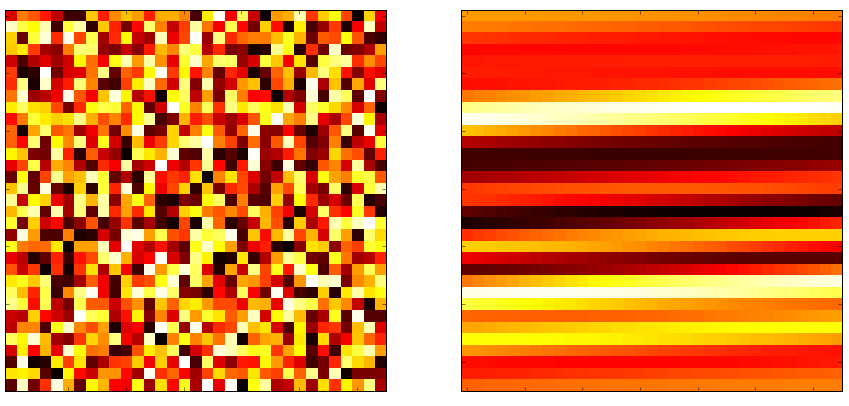
\includegraphics[scale=0.35]{../pictures/DCT-my-case-cropped.png}\\
                \caption{Kompressionsrate 1:55 mit DCT}\label{fig:dct-my-case}
            \end{center}
        \end{figure}

        \noindent
        Man erkennt eine extreme Korrelation zwischen benachbarten Gewichten die der Reihe nach das KNN befüllt haben. Die folgenden drei Algorithmen benutzen die Kompression:

        \begin{itemize}
            \setlength\itemsep{1em}
            \item \textbf{Cross Entropy} (\ref{cross-entropy-definition}) \\
            Hier haben wir die 20 Koeffizienten als Normalverteilung kodiert, $25\%$ der Population als Eltern gewählt und die restlichen $75\%$ aus den neu berechneten Normalverteilungen der Eltern gesamplet. Die Grenzen zum Erstellen der Normalverteilung waren $\mu = 0$ und $\sigma \in [-1.5,1.5]$.

            \item \textbf{Neuroevolution} (\ref{neural-evo-definition}) \\
            Bei der naiven Neuroevolution hat jedes Individuum die 20 Koeffizienten als Zahlen gespeichert. $25\%$ der Population wurden als Eltern gewählt die $50\%$ Kinder erzeugen und die restlichen $25\%$ wurden völlig neu erstellt. Die Grenzen zur Erstellung der Koeffizienten war $c \in [-3,3]$.

            \item \textbf{CoSyNE} (\ref{cosyne-definition}) \\
            Der CoSyNE Algorithmus benutzt die gleichen Ablauf wie Neuroevolution, mit der Ausnahme, dass er statt neue Individuen zu erstellen, genug Kinder erstellt und dann die gesamte Population im Eigenschaftsraum zufällig vermischt.

        \end{itemize}

\newpage

\chapter{Resultate}
    Im folgenden Teil beschreiben wir die Resultate und versuchen diese zu begründen. Durchschnittlich hat eine Trainigsphase mit 300 Generationen, Population der Größe 50 und 25 Episoden pro Team 30 Stunden gedauert. Der Suchraum für die Neuroevolution wurde von 1108Gewichten auf 20 Koeffizienten reduziert, welches einer Kompressionsrate 1:55 entspricht. Die Simulationen wurden auf einem Laptop mit einem Intel i5 mit Dual Core 2.9GHz und 4GB Arbeitsspeicher ausgeführt.\\[2mm]
    \noindent
    Nachdem wir pro Algorithmus die besten 5 Individuen ermittelt haben, ließen wir sie jeweils 10000 Spiele spielen, um die erfasste Fitness auf ihre Stabilität zu testen. Wir haben sie wie folgt quantifiziert:\\[2mm]
%        \noindent
%        Sei $F_{Training}$ die entwickelte Fitness und $F_{Test}$ die neu getestete Fitness. Die Stabilität wird danach gemessen wie gering die Abweichung von $F_{Test}$ zu $F_{Entwicklung}$ ist. Je kleiner die Abweichung, umso stabiler und sicherer spielt das Individuum.\\

        \begin{figure}[H]
            \begin{mdframed}
                Sei $F_{Training}$ die trainierte Fitness, \\
                \hspace*{4mm} $F_{Test}$ die neu getestete Fitness, dann ist der Fehler definiert als:\\[4mm]
                \hspace*{40mm} \Resize{5cm}{$Fehler = \frac{F_{Entwicklung} - F_{Test}}{F_{Entwicklung}}$}
            \end{mdframed}
            \renewcommand{\figurename}{Definition}
            \caption{Berechnung des Fehlers für ein Individuum}
        \end{figure}

        \noindent
        Je kleiner die Abweichung zwischen dem Training und dem Test, umso kleiner ist der Fehler und daher können wir schließen, dass das Individuum sicherer seine versprochene Leistung bringt.\\

        Unser Lernziel für die HFO Domäne war einen offensiven Spieler zu trainieren der gegen einen vom Server gesteuerten Torwart so gut es geht Tore schießt. Das haben wir mit vier in Kapitel 2 angesprochenend Algorithmen getestet und stellen die Resultate vor. \\[2mm]

        \noindent
        Als stabilster und bester Algorithmus ist die naive Neuroevolution mit einer durchschnittlichen Gewinnrate von \textbf{42\%} im Training und \textbf{20\%} im Test. Auf Platz 2 kam CoSyNE mit $37\%$ im Training und $12\%$ im Test. Cross Entropy und die Wahrscheinlichkeitsverteilung der Aktionen haben zwar beide im Training $30\%$ erreicht, aber im Test nur knapp $6\%$ und sind damit extren instabil.
\newpage
            \section{Wahrscheinlichkeitsverteilung der Aktionen}
                \begin{multicols}{2}
                    \noindent
                    Die Wahrscheinlichkeitsverteilung war der erste Ansatz um zu überprüfen ob die Domäne bereits durch eine einfache Kodierung lösbar ist. Leider ging die Varianz in der Population nach der $10$ Generation gegen $0$ und die Verteilung sah folgendermaßen aus:
                    \begin{table}[H]
                        \begin{center}
                        \begin{tabular}{ |l|r| } 
                            \hline
                            \hfill Aktionen & P(Aktion)  \\ \hline
                            Move      & 22\% \\ \hline
                            Dribble   & 22\% \\ \hline
                            Intercept & 22\% \\ \hline
                            No-Op     & 22\% \\ \hline
                            Shoot     &  2\% \\ \hline
                        \end{tabular}
                        \end{center}
                    \end{table}

                    \begin{figure}[H]
                        \centering
                        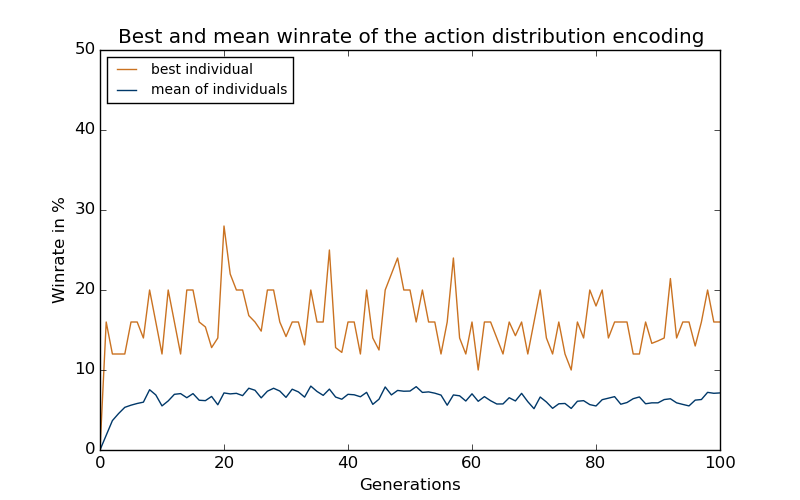
\includegraphics[scale=0.5]{../pictures/summary/actiondist-fitness.png}\\
                        \caption{Fitness Graph für die \\Wahrscheinlichkeitsverteilung}\label{fig:graph-ac}
                    \end{figure}
                \end{multicols}
                \noindent
                Die gesamte Population ist zu dem Ergebnis konvergiert, dass jede Aktion gleich wahrscheinlich ist, bis auf \textit{Shoot}. Die Schussaktion hat wahrscheinlich zu oft zu einem Schuss ins Aus geführt, was sofort das Spiel als verloren wertet.\\

                \noindent
                Die maximale erreichte Fitness beträgt \textbf{33\%} und schwankt eher im Bereich von $[15,25]$. Leider stellt sich heraus, dass die besten Agenten Ausreißer waren und keinesfalls die durchschnittliche Gewinnwahrscheinlichkeit darstellen. \\[4mm]

                \begin{table}[H]
                    \begin{center}
                    \begin{tabular}{ |l|r|r|r| } 
                        \hline
                        \hfill & Trained Fitness   & Tested Fitness   &          Error    \\ \hline
                          Nr.1 &          33.33\%  &          5.26\%  &          82.22\%  \\  
                          Nr.2 &          29.41\%  &          8.87\%  &          70.52\%  \\  
                          Nr.3 &          28.00\%  &          6.06\%  &          78.36\%  \\ 
                          Nr.4 &          25.00\%  &          2.18\%  &          91.28\%  \\ 
                          Nr.5 &          24.00\%  &          6.42\%  &          73.25\%  \\ \hline
                          Mean &  \textbf{27.95\%} &  \textbf{5.72\%}  & \textbf{79.53\%} \\ \hline
                    \end{tabular}
                    \end{center}
                    \caption{Stabilität der besten 5 Individuen \label{fig:actiondisttable}}
                \end{table}
                \noindent
                Die durchschnittliche Gewinnwahrscheinlichkeit liegt bei 5.72\% und wenn man den Spieler beobachtet, kann man sich beim besten Willen nicht erklären, wie er es überhaupt schafft Tore zu schießen, da er meistens versucht ins Tor zu laufen während ihm der Ball abgenommen wird. Das ist aber auch nicht verwunderlich, da der Spieler weder weiß, wo der Torwart ist, noch ob er den Ball hat, oder wo er sich auf dem Spielfeld befindet. \\

\newpage
        \subsubsection*{Illustration eines Torversuchs für einen der Top 5 Agenten}
        \begin{figure}[H]
            \begin{center}
                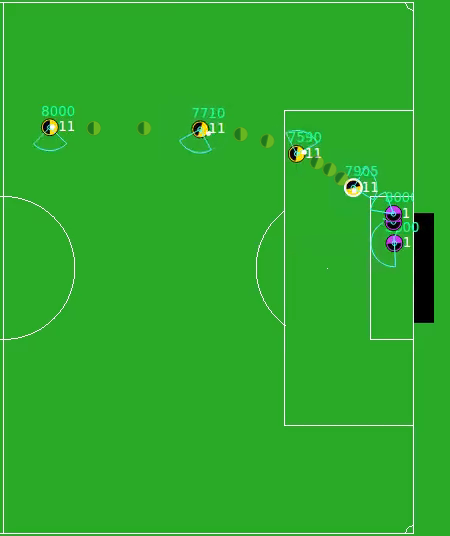
\includegraphics[scale=0.83]{../pictures/games/actiondist-gameplay.png}\\
                \caption{\label{fig:actiondist-gameplay}}
            \end{center}
        \end{figure}

        In Abbildung \ref{fig:actiondist-gameplay} sehen wir einen vielversprechenden Torversuch von dem Individuum. Leider läuft er einfach nur in den Torwart rein und ihm wird sein Ball abgenommen. Es passiert auch sehr oft, dass er vor dem Tor stehen bleibt, oder einfach nur wild um sich herumschießt, egal in welcher Position er steht. Aus der Tabelle der Verteilungen kann man nur bestätigen dass sich sein Verhalten zufällig beschreiben lässt.


\newpage
            \section{Cross Entropy}
                \begin{multicols}{2}
                    \noindent
                    \\[5mm]
                    Die Cross Entropy Methode hat nach der statistischen Analyse keine besonders unterschiedliche Werte produziert, da sie durchschnittlich eine 2\% bessere Fitness hat und die Stabilität um 1\% besser ist, als wie die Wahrscheinlichkeitsverteilung.\\[2mm]
                    Sie ist nach ungefähr 50 Generationen konvergiert, die maximale erreichte Fitness beträgt \textbf{32\%} und schwankt im Bereich von $[15,30]$. 
                    \begin{figure}[H]
                       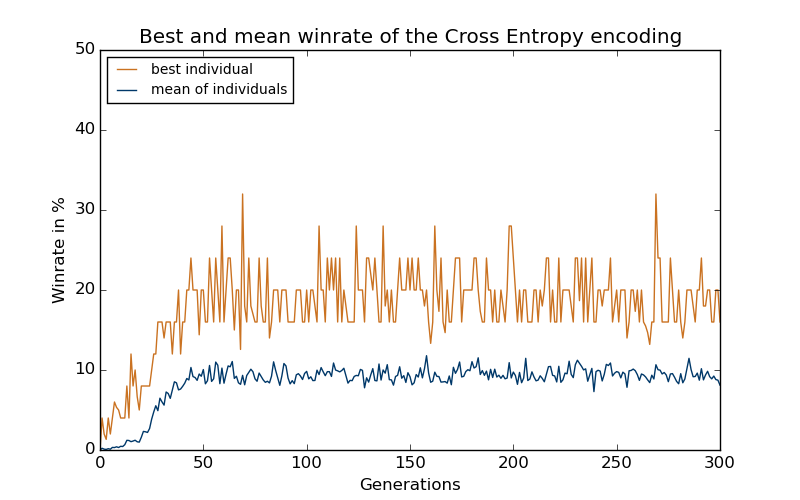
\includegraphics[scale=0.5]{../pictures/summary/cross-entropy-fitness.png}
                       \caption{Fitness Graph für Cross Entropy}\label{fig:graph-ce}
                    \end{figure}
                \end{multicols}

                \begin{table}[H]
                    \begin{center}
                    \begin{tabular}{ |l|r|r|r| } 
                        \hline
                        \hfill & Trained Fitness   & Tested Fitness  &          Error    \\ \hline
                          Nr.1 &          32.00\%  &          7.26\% &          77.31\%  \\  
                          Nr.2 &          32.00\%  &          7.46\% &          76.69\%  \\  
                          Nr.3 &          28.00\%  &          7.37\% &          73.68\%  \\ 
                          Nr.4 &          28.00\%  &          7.27\% &          74.04\%  \\ 
                          Nr.5 &          28.00\%  &          3.46\% &          87.64\%  \\ \hline
                          Mean &  \textbf{29.60\%} & \textbf{6.56\%} & \textbf{77.87\%}  \\ \hline
                    \end{tabular}
                    \end{center}
                    \caption{Stabilität der besten 5 Cross Entropy Individuen \label{fig:crossentropytable}}
                \end{table}
                \noindent
                Von den Werten sieht man kaum einen Unterschied zu der Wahrscheinlichkeitsverteilung, aber in der Simulation merkt man ein extrem aggressives Verhalten vom Spieler. Der Agent schießt den Ball sehr oft und versucht bereits nachdem er die Mitte des Spielfeldes überquert hat ein Tor zu schießen, unabhängig davon ob er in einer guten Position ist. Das führt natürlich dazu dass er öfter ins Aus schießt, ist aber wesentlich interessanter anzuschauen, da er jedes Spiel unberechenbar ist. \\[2mm]

                \noindent
                Es ist zu beachten, dass dieser Algorithmus die \textbf{schnellste Lernkurve} von den drei Algorithmen hatte, die im komprimierten DCT Raum arbeiten.
\newpage
                \subsubsection*{Illustration eines Torversuchs für einen der Top 5 Agenten}
                \begin{center} \textit{Beispielhafte Abfolge von einem Spiel für den Cross Entropy Method} \end{center}
\newpage
            \section{Neuroevolution}
                \begin{multicols}{2}
                    \noindent
                    \\[5mm]
                    Der Ansatz die Gewichte naiv als DCT Koeffizienten darzustellen, führte zu den besten Ergebnissen. Das stärkste Individuum hat knapp \textbf{jedes zweite Spiel gewonnen} und ist mehr als 3-mal stabiler als die Cross-Entropy Lösung. Die Fitness hat sich nach ungefähr 150 Generationen im Bereich von $[30,45]$ eingependelt.
                    \begin{figure}[H]
                       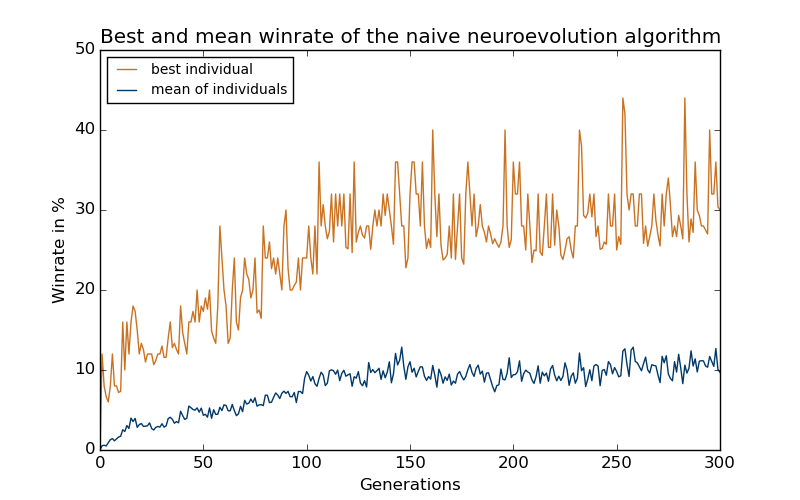
\includegraphics[scale=0.5]{../pictures/summary/neural-fitness.png}
                       \caption{Fitness Graph für Cross Entropy}\label{fig:graph-ne}
                    \end{figure}
                \end{multicols}

                \begin{table}[H]
                    \begin{center}
                    \begin{tabular}{ |l|r|r|r| } 
                        \hline
                        \hfill & Trained Fitness   & Tested Fitness  &          Error    \\ \hline
                          Nr.1 &          44.00\%  &         19.04\% &          56.72\%  \\  
                          Nr.2 &          44.00\%  &         20.18\% &          54.14\%  \\  
                          Nr.3 &          42.00\%  &         20.07\% &          52.21\%  \\ 
                          Nr.4 &          40.00\%  &         20.10\% &          49.75\%  \\ 
                          Nr.5 &          40.00\%  &         21.28\% &          46.80\%  \\ \hline
                          Mean &  \textbf{42.00\%} & \textbf{20.13\%} & \textbf{51.93\%}  \\ \hline
                    \end{tabular}
                    \end{center}
                    \caption{Stabilität der besten 5 Individuen \label{fig:neuroevotable}}
                \end{table}

                \noindent
                Die stabile Fitness ist bei knapp 20\% und damit gewinnen diese Individuen durchschnittliche jedes fünfte Spiel. Hier haben wir bereits starke Anzeichen für eine Taktik gesehen. Der Agent rennt von Anfang an zum Tor, bleibt kurz vor dem Strafraum stehen und pendelt von Ecke zu Ecke bis der Torwart weiter rausgeht um ein Tor zu schießen.\\

                \noindent
                Wenn er mal verliert, ist es weil er sofort zum Beginn des Spieles sich ins Aus schießt, oder zu nah am Tor ist, sodass ihm der Ball abgenommen wird. Die Tendenz am Ende des Graphen deutet darauf hin, dass bei längeren Laufzeiten noch bessere Ergebnisse möglich wären.% Die stichprobenartigen Aufnahmen von diesen Agenten haben dennoch Gewinnserien von 3-4 Spielen hintereinander gezeigt, obwohl die die Wahrscheinlichkeit dafür 
\newpage
        \subsubsection*{Illustration eines Torversuchs für einen der Top 5 Agenten}
        \begin{figure}[H]
            \begin{center}
                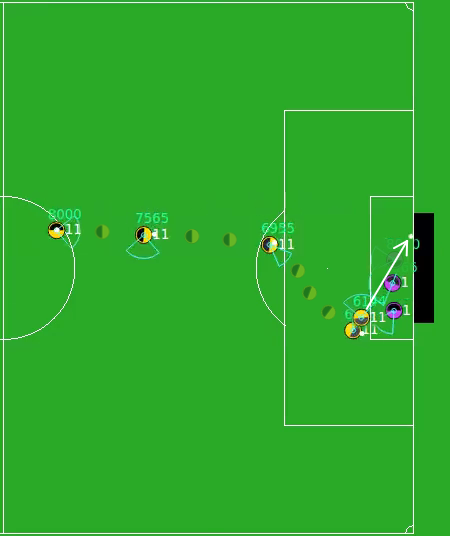
\includegraphics[scale=0.83]{../pictures/games/neural-evo-gameplay.png}\\
                \caption{\label{fig:neural-evo-gameplay}}
            \end{center}
        \end{figure}
        In Abbildung \ref{fig:neural-evo-gameplay} sehen wir die bisher interessanteste Bewegung, da der Agent versucht sich zuerst in die untere Ecke zu positionieren, dabei den Torwart etwas rauslockt, um dann haarfein das Tor zu schießen. Diese Taktik ist die ausgereifteste, da sie die Reaktion des Torwarts, der Abhängigkeit des größsten offenen Winkels zum Tor und der damit in Beziehung stehende Torchancen in Betracht zieht. Aus anderen Visualisierungen haben wir auch Tore außerhalb des Strafraums fallen sehen, was bedeutet dass der Agent nicht nur eine einzelne Gewinnstrategie gelernt hat, sondern wirklich \textit{abwägt}, welche Aktion gerade am nützlichsten ist.
\newpage
            \section{CoSyNE}
                \begin{multicols}{2}
                    \noindent
                    \\[5mm]
                    Der CoSyNE Algorithmus ist in der durchschnittlichen Fitness knapp 5\% hinter der Neuroevolution, hat dafür aber ganze 15\% in der Stabilität verloren. Aus der Natur von dem CoSyNE gab es selbst bei der 300 Generation noch exterm unterschiedliche Individuen und eine Konvergenz war nicht zu erkennen. 
                    \begin{figure}[H]
                       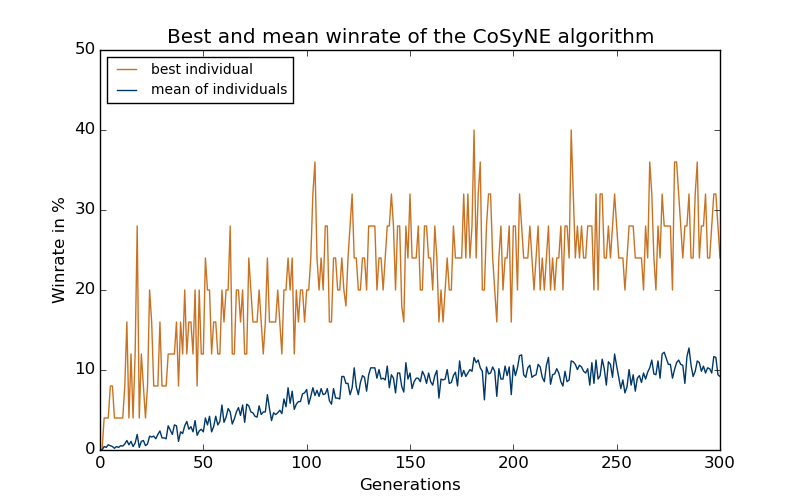
\includegraphics[scale=0.5]{../pictures/summary/cosyne-fitness.png}
                       \caption{Fitness Graph für Cross Entropy}\label{fig:graph-co}
                    \end{figure}
                \end{multicols}

                \begin{table}[H]
                    \begin{center}
                    \begin{tabular}{ |l|r|r|r| } 
                        \hline
                        \hfill & Trained Fitness   & Tested Fitness  &          Error    \\ \hline
                          Nr.1 &          40.00\%  &         14.21\% &          64.47\%  \\  
                          Nr.2 &          40.00\%  &         14.22\% &          64.45\%  \\  
                          Nr.3 &          36.00\%  &         12.68\% &          64.48\%  \\ 
                          Nr.4 &          36.00\%  &         15.42\% &          57.16\%  \\ 
                          Nr.5 &          36.00\%  &          5.75\% &          84.02\%  \\ \hline
                          Mean &  \textbf{37.60\%} & \textbf{12.45\%} & \textbf{66.98\%}  \\ \hline
                    \end{tabular}
                    \end{center}
                    \caption{Stabilität der besten 5 Neurevolution Individuen \label{fig:neuroevotable}}
                \end{table}
                \noindent
                Die beste Individuen haben lediglichlich nur knapp 12\% ihrer Spiele gewonnen und man kann eine ähnliche Taktik wie die Neuroevolution Agenten erahnen, nur wesentlich schlechter umgesetzt. Es passiert häufig, dass der Agent kurz vor dem Strafraum stehen bleibt und sich für eine sehr lange Zeit nicht bewegt. Da der Torwart nicht zu weit von dem Tor rausgeht, befinden sie sich im Deadlock bis der Agent versucht ein Tor zu schießen. Das Schießen ins Aus am Anfang des Spiels tritt hier gehäuft auf.\\

                \noindent
                Eine interessante Eigenschaft von CoSyNE ist das stufenartige Entwickeln der Fitness die ab bestimmten Generationen nie wieder schlechter wird.

\newpage
                \subsubsection*{Illustration eines Torversuchs für einen der Top 5 Agenten}
                \begin{center} \textit{Beispielhafte Abfolge von einem Spiel für CoSyNE} \end{center}
\newpage

        \section{Vergleich} \label{algo-comparisson}
             Im Vergleich zwischen allen Algorithmen sieht das Ranking folgendermaßen aus:

                \begin{table}[H]
                    \begin{center}
                    \begin{tabular}{ |l|r|r|r| } 
                        \hline
                        \textbf{Algorithmus}          & E(Trained Fitness) & E(Tested Fitness) & E(Error)    \\ \hline
                        Neuroevolution                &          42.00\%   &         20.13\%   &    51.93\%  \\ \hline
                        CoSyNE                        &          37.60\%   &         12.45\%   &    66.98\%  \\ \hline
                        Cross-Entropy                 &          29.60\%   &          6.56\%   &    77.87\%  \\ \hline
                        Wahrscheinlichkeitsverteilung &          24.60\%   &          6.15\%   &    74.88\%  \\ \hline
                    \end{tabular}
                    \end{center}
                    \caption{Alle Algorithmen gegenübergestellt \label{fig:vergleichstabelle}}
                \end{table}

            \noindent
            Neuroevolution gewinnt eindeutig in allen getesteten Merkmalen und hat während den Aufnahmen den raffiniertesten Eindruck gemacht. Wir sehen, dass die Aggressivität bei der Cross-Entropy Method zwar interessante Züge macht, jedoch nicht tauglich für den Einsatz auf dem echten Spielfeld ist. \\[2mm]

            \noindent
            Sicherheit und die \textit{Planung} machen auf lange Sicht viel mehr Sinn und sollten verstärkt werden. Der CoSyNE Algorithmus unterstützt diese Art von Entwicklung in dieser Dimensionalität schlechter als die naive Suche über alle Parameter. Es ist zu überprüfen ob diese Aussage für gleichzeitiges Lernen in einem 2v1 Setting übereinstimmt.\\[2mm]

            \begin{center} \textit{(Link zur Best-Of-Compilation Video)} \end{center}